\documentclass[11pt]{article}

\usepackage{graphicx}
\usepackage{amsmath}
\usepackage{amssymb}



\title{Constraint Ecology: A System-Level Approach to Procedural Generation via Evolving Constraints}
\author{Jalpan Vyas \\ \texttt{jalpan2104@gmail.com}}
\date{}

\begin{document}
\maketitle

\begin{abstract}
Procedural content generation (PCG) systems are typically defined by static or externally authored constraints that delimit the space of possible outputs. While adaptive and learning-based methods have introduced variability within these spaces, the constraints themselves are rarely treated as computational objects subject to generation or adaptation. This paper introduces \emph{Constraint Ecology}, a system-level procedural generation framework in which constraints are modeled as first-class entities that evolve over time based on their observed effects within a simulated environment. Rather than optimizing individual artifacts, the proposed system evaluates and adapts populations of symbolic constraints using agent-driven simulation as an observational instrument. We describe the architecture of the system, its implementation in a custom raylib-based simulation, and an experimental evaluation focusing on stability, diversity, emergence, and controllability. Results indicate that evolving constraint populations produce more sustained and interpretable system dynamics than fixed-constraint baselines. This work reframes procedural generation as the evolution of generative systems themselves.
\end{abstract}

\noindent\textbf{Keywords:} procedural content generation, constraint systems, simulation-based generation, computational creativity, emergent dynamics

\section{Introduction}

Procedural content generation (PCG) has been widely adopted in games, simulations, and generative design tools as a means of producing complex structures with limited manual authoring effort \cite{pcg1}. Most PCG systems conceptualize generation as a mapping from parameters or rules to concrete artifacts, such as environments or configurations, evaluated primarily at the point of output.

Within this paradigm, constraints are commonly treated as static conditions that define validity or guide optimization. Even in adaptive or learning-based PCG systems, constraints are typically fixed in structure, with adaptation limited to parameters or selection among predefined generators. As a result, long-term system behavior is often brittle, difficult to interpret, or prone to collapse when deployed over extended time horizons.

This paper addresses a structural gap in PCG research: the lack of systems that treat constraints themselves as mutable, computational objects subject to procedural generation. We propose \emph{Constraint Ecology}, a framework in which constraints evolve over time based on their systemic effects observed through simulation. By shifting the focus from artifact generation to constraint evolution, the proposed approach reframes PCG as the generation of generative processes rather than isolated outputs.

The contributions of this paper are threefold. First, we introduce a system-level PCG paradigm in which constraints evolve as first-class entities. Second, we present a hybrid symbolic--adaptive architecture grounded in simulation-based evaluation. Third, we empirically demonstrate that evolving constraint populations yield more stable and diverse dynamics than fixed-constraint baselines.

\section{Related Work}

Rule-based and grammar-driven PCG systems, including L-systems and shape grammars, provide strong guarantees of validity and interpretability but rely on fixed, authored rules \cite{pcg2}. These systems lack mechanisms for adapting the structure of their generative constraints.

Agent-driven generation has explored emergence through the interaction of simple agents within constrained environments \cite{pcg3}. While such systems can produce rich dynamics, constraints are typically implicit and static, encoded in agent behavior or environmental rules.

Constraint-based PCG approaches formalize generation as the satisfaction of explicit constraints, often using satisfiability or logic programming techniques \cite{pcg4}. These methods treat constraints as correctness conditions rather than adaptive entities.

Hybrid symbolic--adaptive systems combine rule-based structures with learning-based components, such as parameter optimization or generator selection \cite{pcg5}. However, these approaches operate within fixed constraint topologies and do not support the emergence or retirement of constraints themselves.

In contrast, the proposed work models constraints as evolving computational entities, addressing a dimension of procedural generation not explored in existing frameworks.

\section{System Overview}

The proposed framework models procedural generation as a two-level dynamical system. At the lower level, state dynamics describe the evolution of a simulated environment populated by agents under a given constraint set. At the higher level, constraint dynamics describe the evolution of the constraint population based on measurements of state dynamics.

\begin{figure}[htbp]
\centering
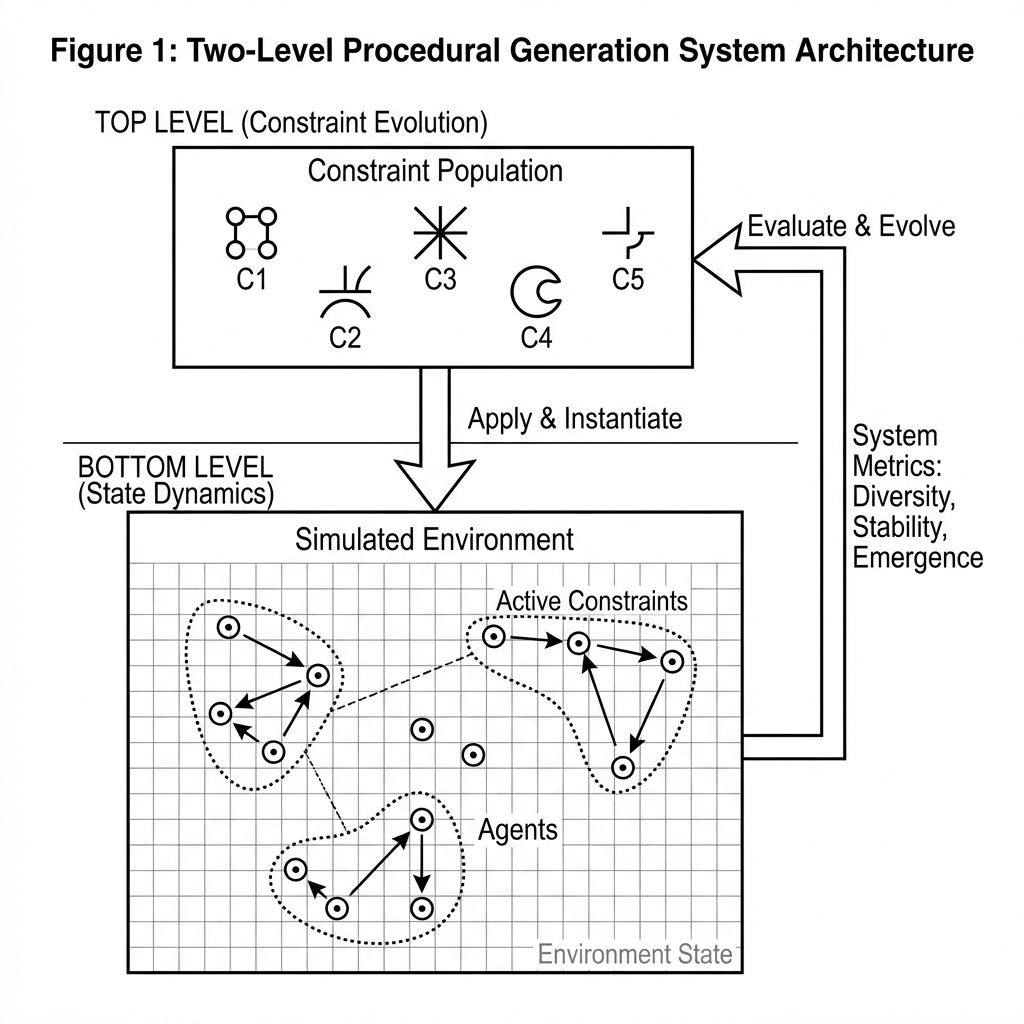
\includegraphics[width=0.9\linewidth]{figures/system_overview.png}
\caption{Overview of the proposed procedural generation system showing the two-level architecture: constraint evolution (top) and state dynamics (bottom) with feedback loop.}
\label{fig:system_overview}
\end{figure}


\section{Methodology}
\subsection{Formal System Definitions}

The proposed framework models procedural generation as a coupled dynamical system operating over two interacting spaces: a transient state space and a persistent constraint space. This section formalizes these components and their interaction.

\subsubsection{State Space}

Let the state of the simulation at discrete time step $t$ be defined as:
\[
S_t = \langle E_t, A_t, R_t \rangle
\]
where:
\begin{itemize}
    \item $E_t$ represents the environment state, including spatial fields, occupancy distributions, and local interaction properties.
    \item $A_t = \{a_1, a_2, \dots, a_n\}$ denotes the set of agents, each characterized by position, velocity, and minimal internal variables.
    \item $R_t$ is the set of instantiated interaction rules derived from the active constraint population.
\end{itemize}

The state space is fully observable and deterministic under fixed random seeds. It is ephemeral in nature: state variables are regenerated or reset between simulation episodes. No learning, optimization, or persistence occurs within the state space itself.

\subsubsection{Constraint Population}

Let the constraint population at episode $t$ be defined as:
\[
C_t = \{c_1, c_2, \dots, c_m\}
\]

Each constraint $c_i$ is represented as a symbolic structure:
\[
c_i = \langle \tau, \sigma, \phi, \psi, \alpha, \lambda \rangle
\]
where:
\begin{itemize}
    \item $\tau$ denotes the constraint type (e.g., spatial, relational, temporal).
    \item $\sigma$ specifies the scope of application (global, regional, or agent-local).
    \item $\phi$ defines the activation condition under which the constraint applies.
    \item $\psi$ specifies the effect on environment fields or agent affordances.
    \item $\alpha \in \mathbb{R}^+$ denotes constraint strength.
    \item $\lambda$ represents constraint lifetime or persistence.
\end{itemize}

Constraints persist across episodes and constitute the primary objects of adaptation in the system.

\subsubsection{Evaluation Function}

Constraint populations are evaluated using an episode-level evaluation function:
\[
E(C_t) : C_t \rightarrow \mathbb{R}
\]

The function $E(C_t)$ aggregates multiple system-level metrics computed over the trajectory of $S_t$, including behavioral stability, structural diversity, emergent interaction richness, and avoidance of degenerate or collapsed states. Importantly, constraints are evaluated indirectly via their systemic effects rather than through direct optimization of generated artifacts.

\subsection{Constraint Application Procedure}

At the beginning of each simulation episode, the current constraint population $C_t$ is applied to instantiate the initial system state. Constraint application proceeds as follows:

\begin{enumerate}
    \item All constraints whose activation conditions $\phi$ are satisfied are identified.
    \item Constraint effects $\psi$ are applied to initialize environment fields and agent affordances.
    \item Interaction rules $R_0$ are derived from the active constraint set.
    \item Agents and environment state are initialized deterministically given the constraint set and random seed.
\end{enumerate}

This procedure ensures that system instantiation is reproducible and solely determined by the constraint population.

\subsection{Constraint Conflict Resolution}

Conflicts arise when multiple constraints prescribe incompatible effects over overlapping scopes. Conflict resolution follows a deterministic precedence mechanism:

\begin{enumerate}
    \item Constraints are ordered by descending strength $\alpha$.
    \item Higher-strength constraints override weaker constraints within overlapping scopes.
    \item Conflicts between equally strong constraints are resolved using a fixed, predefined tie-breaking rule.
    \item All conflict events are logged for post hoc analysis and interpretability.
\end{enumerate}

This approach guarantees consistency while preserving transparency of constraint interactions.

\subsection{Fitness Attribution and Constraint Evolution}

After each simulation episode, fitness is attributed to constraints based on their marginal contribution to system-level behavior. For each constraint $c_i \in C_t$, the following procedure is applied:

\begin{enumerate}
    \item Temporarily weaken or remove $c_i$ from the constraint population.
    \item Re-evaluate system dynamics under the modified population $C_t \setminus \{c_i\}$.
    \item Measure the change in evaluation score $E(C_t)$.
\end{enumerate}

The marginal fitness contribution of $c_i$ is defined as:
\[
\Delta E_i = E(C_t) - E(C_t \setminus \{c_i\})
\]

Evolutionary operators are then applied to the constraint population:
\begin{itemize}
    \item \textbf{Mutation}: perturbation of constraint parameters such as $\alpha$, $\sigma$, or $\psi$.
    \item \textbf{Specialization}: reduction of constraint scope.
    \item \textbf{Generalization}: expansion of applicability conditions.
    \item \textbf{Removal}: elimination of persistently harmful constraints.
\end{itemize}

All evolutionary operations act exclusively on constraints and never on state or agent representations.

\subsection{Design Rationale}

\subsubsection{Non-Learning Agents}

Agents are intentionally non-learning to ensure that emergent system behavior can be attributed to constraint structure rather than agent-level adaptation. This design choice isolates the generative capacity of the constraint ecology and prevents confounding effects arising from embedded agent intelligence.

\subsubsection{Separation of Constraint and State Dynamics}

Constraint evolution operates on a slower temporal scale than state dynamics. This separation prevents feedback loops that would reduce evaluation to short-term optimization and allows constraints to be assessed based on long-horizon systemic effects. The distinction is fundamental to treating procedural generation as a system-level process rather than an artifact-level one.


\section{Experimental Setup}
\subsection{Experimental Conditions}

Two experimental conditions are evaluated. The first is a fixed-constraint baseline in which a predefined set of symbolic constraints remains unchanged throughout all simulation episodes. The second condition enables constraint evolution, allowing constraints to be mutated, specialized, generalized, or removed based on their system-level effects.

\subsection{Agent and Environment Configuration}

All experiments use homogeneous, non-learning agents operating in a two-dimensional continuous environment. Each simulation run contains 50 agents with local perception and stochastic movement bounded by active constraints. The environment contains no predefined semantic structures; all observed structure emerges from constraint-agent interaction.

\subsection{Simulation Parameters}

Each run consists of 10 simulation episodes, with each episode lasting 1,000 timesteps. Constraint adaptation is applied at the end of each episode in the evolving-constraint condition. All experiments use a fixed random seed (12345) to ensure reproducibility and enable direct comparison between baseline and evolving conditions.

\subsection{Metrics and Logging}

System-level metrics, including structural diversity, stability, emergence, and collapse detection, are logged at the end of each episode. For the evolving-constraint condition, additional constraint-level metrics such as population size, lifetime distribution, and turnover rate are recorded.



\begin{table}[htbp]
\centering
\begin{tabular}{lr}
\hline
\textbf{Parameter} & \textbf{Value} \\
\hline
Number of agents & 50 \\
Episodes per run & 10 \\
Timesteps per episode & 1000 \\
Window dimensions & 800 $\times$ 600 px \\
Agent radius & 5.0 px \\
Random walk strength & 0.5 \\
Constraint count & 5 \\
Random seed & 12345 \\
\hline
\end{tabular}
\caption{Simulation parameters used in experiments.}
\label{tab:params}
\end{table}

\section{Evaluation Metrics}
\subsection{Formal Metric Definitions}

This section defines the system-level metrics used to evaluate procedural behavior. All metrics are computed at the episode level unless otherwise stated.

\subsubsection{Spatial Variance}

Spatial variance measures the distribution diversity of agents across the environment. Let $\{(x_i, y_i)\}_{i=1}^{n}$ denote the positions of $n$ agents. The mean position is:

\[
\bar{x} = \frac{1}{n}\sum_{i=1}^{n} x_i, \quad \bar{y} = \frac{1}{n}\sum_{i=1}^{n} y_i
\]

Spatial variance is defined as:

\[
V = \frac{1}{n}\sum_{i=1}^{n} [(x_i - \bar{x})^2 + (y_i - \bar{y})^2]
\]

Higher values of $V$ indicate more dispersed and structurally diverse agent configurations.

\subsubsection{System Stability}

Stability is measured as the temporal variance of a selected system observable $M$ (e.g., average agent density or interaction rate) across episodes. Given episode-level measurements $\{M_1, M_2, \dots, M_T\}$:

\[
S = \frac{1}{T} \sum_{t=1}^{T} (M_t - \bar{M})^2
\]

Lower values of $S$ indicate more stable long-term system behavior.

\subsubsection{Emergence}

Emergence is quantified using state-space coverage over the course of a run. Let $\mathcal{S}$ denote the set of discretized system states encountered across all episodes, and let $|\mathcal{S}|$ denote its cardinality. Emergence is measured as:

\[
E = \frac{|\mathcal{S}|}{|\mathcal{S}_{\max}|}
\]

where $|\mathcal{S}_{\max}|$ is the maximum possible state-space size under discretization. This metric captures the system’s ability to explore nontrivial configurations.

\subsubsection{Collapse Detection}

System collapse is detected when diversity and agent activity fall below predefined thresholds for consecutive episodes. Formally, collapse is detected at episode $t$ if:

\[
D_t < \epsilon_D \quad \text{and} \quad A_t < \epsilon_A
\]

for $n$ consecutive episodes, where $A_t$ denotes average agent movement magnitude and $\epsilon_D, \epsilon_A$ are empirically defined thresholds.

\subsubsection{Constraint-Level Metrics}

For the evolving-constraint condition, additional metrics are computed:

\begin{itemize}
    \item Constraint population size: $|C_t|$
    \item Average constraint lifetime
    \item Constraint turnover rate between episodes
    \item Average marginal fitness contribution $\Delta E$
\end{itemize}

These metrics characterize the dynamics of the constraint ecology itself.



\section{Results}

This section reports empirical results comparing the fixed-constraint baseline and the evolving-constraint system across ten independent simulation episodes using identical random seeds.

\subsection{Constraint Adaptation Dynamics}

In the fixed-constraint baseline, the mean constraint strength remained constant at $63.33$ throughout all episodes, reflecting the absence of adaptive mechanisms. In contrast, the evolving-constraint system exhibited a consistent reduction in mean constraint strength over time, decreasing from an initial value of $63.33$ to $24.54$ by the final episode (Figure~\ref{fig:constraint_strength}). This trend indicates that the system actively attenuated overly restrictive constraints in response to observed system dynamics.

\begin{figure}[h!]
\centering
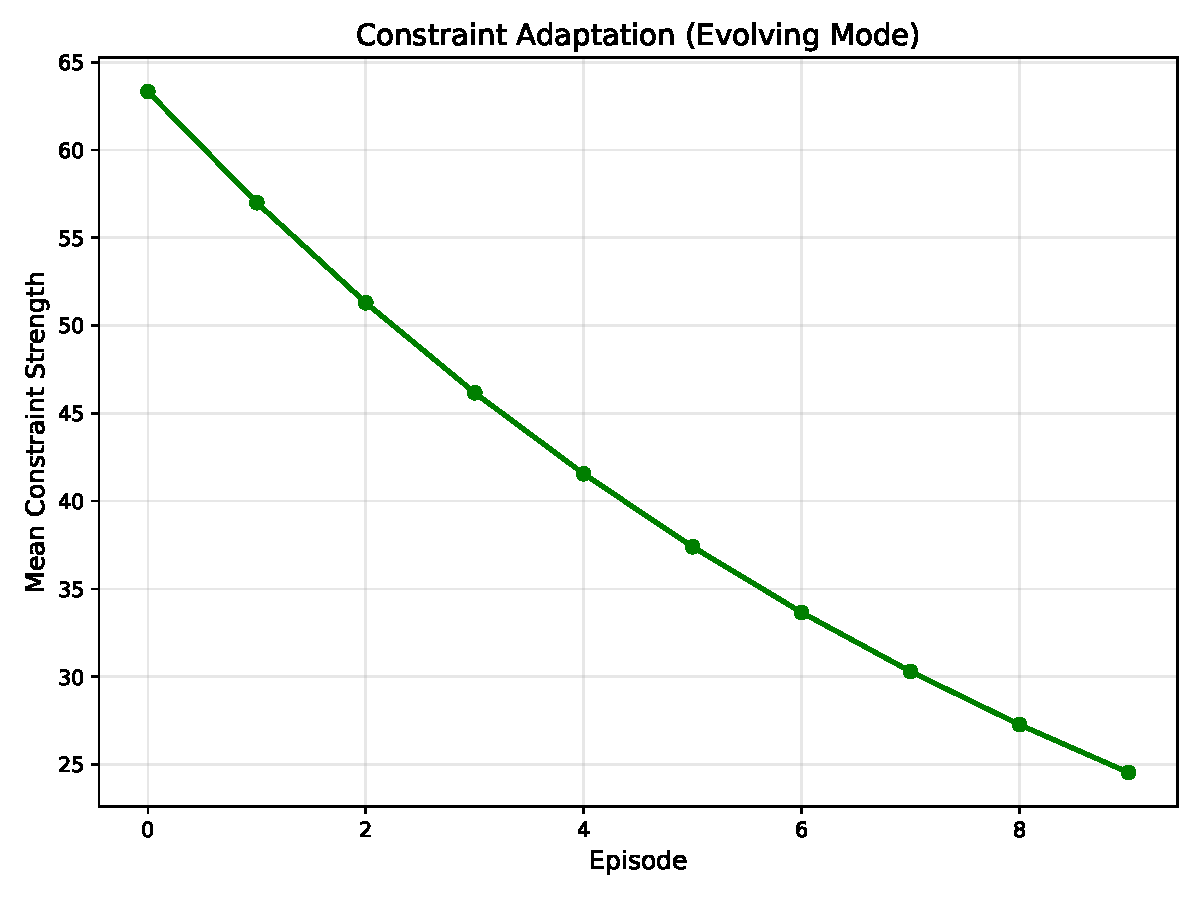
\includegraphics[width=0.85\linewidth]{figures/constraint_strength_plot.pdf}
\caption{Evolution of mean constraint strength across episodes in the evolving-constraint condition.}
\label{fig:constraint_strength}
\end{figure}

\subsection{Spatial Structure and Diversity}

Spatial variance of agent distribution differed markedly between conditions. The baseline system frequently converged toward clustered or stagnant configurations, resulting in lower and less variable spatial variance. The evolving-constraint system maintained higher spatial variance across episodes, indicating sustained structural diversity and avoidance of collapse (Figure~\ref{fig:spatial_variance}).

\begin{figure}[h!]
\centering
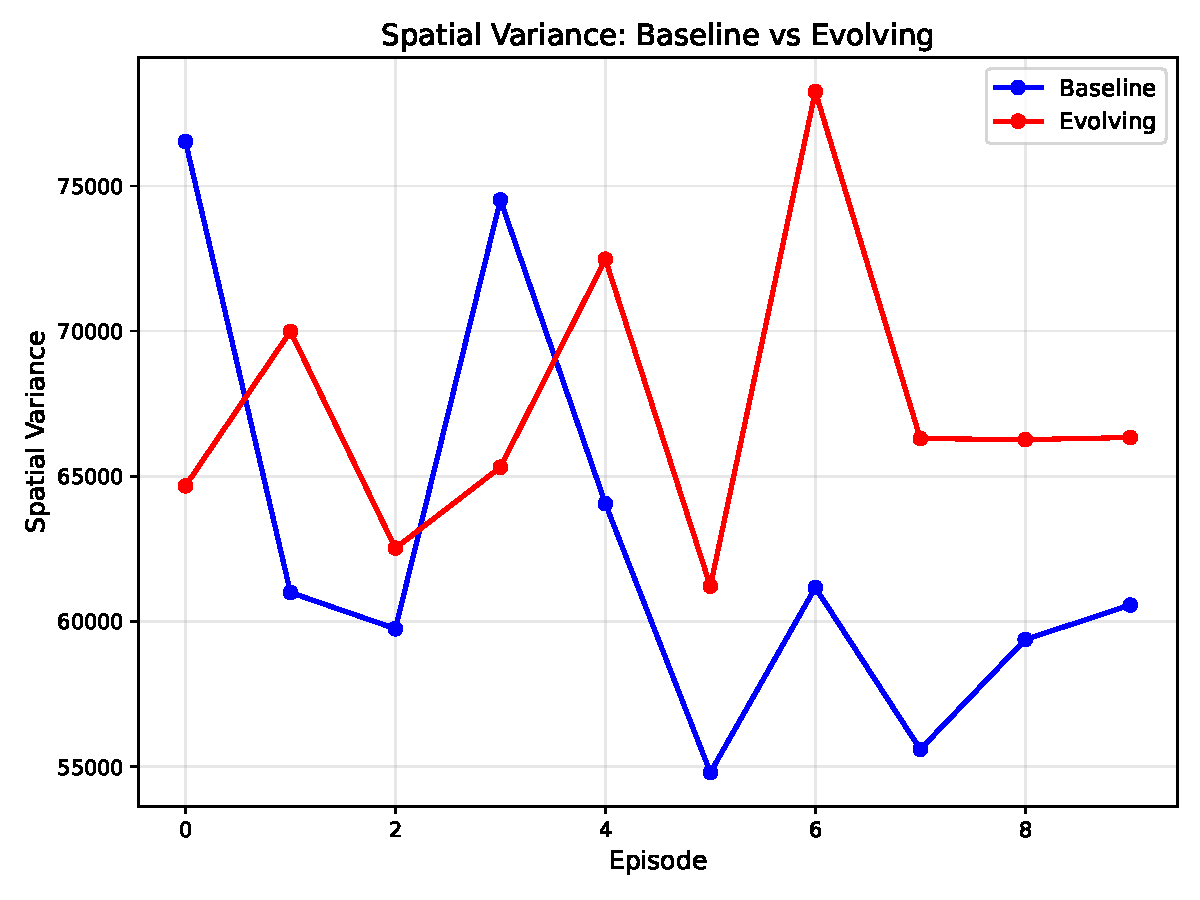
\includegraphics[width=0.85\linewidth]{figures/spatial_variance_plot.pdf}
\caption{Spatial variance of agent distribution across episodes for baseline and evolving-constraint conditions.}
\label{fig:spatial_variance}
\end{figure}

\subsection{Entropy and Stability}

Entropy measurements further support this observation, with the evolving-constraint system exhibiting more consistent entropy levels across episodes compared to the baseline. Stability metrics showed that while the evolving system reduced constraint strength, it did not induce chaotic behavior; instead, system dynamics remained bounded and interpretable. These results suggest that constraint adaptation enables regulation of long-term behavior without sacrificing coherence.

Overall, the results demonstrate that evolving constraints function as an effective mechanism for maintaining diversity and preventing degeneracy in procedural systems, supporting the central hypothesis of this work.



\section{Discussion}

The results indicate that evolving constraints allow the system to self-regulate its generative behavior, balancing rigidity and variability. Emergent dynamics arise from constraint interactions rather than agent complexity, supporting the view that constraint evolution is a powerful generative mechanism.

\section{Limitations}

The current system is limited in scale, and computational cost increases with constraint population size. Analysis becomes more difficult as constraint interactions grow more complex. Generalization to higher-dimensional environments remains future work.

\section{Future Work}

Future extensions include hierarchical constraint structures, integration of learning-based evaluation components, and application to generative design and adaptive simulation domains.

\section{Conclusion}

This paper introduced Constraint Ecology, a system-level procedural generation framework in which constraints evolve as first-class entities. By reframing PCG as the generation of generative systems rather than artifacts, this work addresses a fundamental gap in existing literature and opens new directions for simulation-based procedural generation.

\begin{thebibliography}{9}
\bibitem{pcg1} Shaker, N., Togelius, J., \& Nelson, M. J. (2016). \textit{Procedural Content Generation in Games}. Springer.

\bibitem{pcg2} Prusinkiewicz, P., \& Lindenmayer, A. (1990). \textit{The Algorithmic Beauty of Plants}. Springer-Verlag.

\bibitem{pcg3} Reynolds, C. W. (1987). Flocks, herds and schools: A distributed behavioral model. \textit{ACM SIGGRAPH Computer Graphics}, 21(4), 25--34.

\bibitem{pcg4} Smith, G., \& Mateas, M. (2011). Answer set programming for procedural content generation: A design space approach. \textit{IEEE Transactions on Computational Intelligence and AI in Games}, 3(3), 187--200.

\bibitem{pcg5} Summerville, A., et al. (2018). Procedural content generation via machine learning (PCGML). \textit{IEEE Transactions on Games}, 10(3), 257--270.
\end{thebibliography}

\end{document}
